%%% 必須 %%%
\documentclass[dvipdfmx,a4j,11pt]{jsarticle}
\usepackage[left=25truemm,right=25truemm,top=30truemm,bottom=30truemm]{geometry}
\usepackage{amsfonts,amsmath,amssymb,amsthm,bm,cite,enumerate,fancyhdr,multicol,physics}

%%% 図や画像の挿入 %%%
\usepackage[dvipdfmx,hiresbb]{graphicx}

%%% リンクに色 %%%
\usepackage[colorlinks,linkcolor=blue,urlcolor=blue]{hyperref}

%%% しおりの文字化け回避 %%%
\usepackage{pxjahyper}

%%% フォント %%%
\usepackage[T1]{fontenc} 
\usepackage{newtxtext,newtxmath} 

\usepackage[noalphabet]{pxchfon} % JAPANESE FONTS
\setminchofont{msmincho}
\setgothicfont{msgothic}

%%% 色 %%%
\usepackage{xcolor}  %\usepackage{color}
\hypersetup{
    colorlinks=false,
    citebordercolor=green!40,
    linkbordercolor=yellow!40,
    urlbordercolor=cyan!40,
}

%%% 作図 %%%
\usepackage{tikz}
\usetikzlibrary{positioning,arrows,intersections, calc, through}


%%% 見出しカスタマイズ  %%%
\usepackage{titlesec}%%%  \usepackage{newtxtext,newtxmath}の下に書く

\titleformat{\chapter} %\sectionを変更する
   [hang] % 形状
   {\sffamily\huge} %フォント,サイズ
   {第\thechapter 章} %ラベル
   {0zw} %ラベルと見出しとの間
   {\hspace{20pt}} %見出し文字列の前
   [] %見出しの後

\titleformat{\section}[hang]{\sffamily\Large}{\thesection}{0zw}{\hspace{20pt}}[\titlerule\titlerule] 

\titleformat{\subsection}[hang]{\sffamily\large}{\thesubsection}{0zw}{\hspace{4pt}}[\vspace{8pt}]   

%%% 定理環境 %%%
\usepackage[most]{tcolorbox}
\tcbuselibrary{theorems}

\usepackage{cleveref} % !!WARNIG!! BELOW \newtheorem
                          

\renewcommand\proofname{\bf 証明}

\newtcbtheorem[number within=section]{thm}{定理}%
{theorem style=plain,sharp corners,
fonttitle=\sffamily,fontupper=\upshape,before skip=10pt,
colframe=blue!50!white,colback=blue!0!white,
colbacktitle=blue!20!white,coltitle=blue!0!black,
left=2mm,right=2mm,top=0mm,bottom=0mm,boxrule=0.5pt}{theo}

\newtcbtheorem[use counter from=thm]{prop}{命題}%
{theorem style=plain,sharp corners,
fonttitle=\sffamily,fontupper=\upshape,before skip=10pt,
colframe=blue!50!white,colback=blue!0!white,
colbacktitle=blue!20!white,coltitle=blue!0!black,
left=2mm,right=2mm,top=0mm,bottom=0mm,boxrule=0.5pt}{propo}

\newtcbtheorem[use counter from=thm]{cor}{系}%
{theorem style=plain,sharp corners,
fonttitle=\sffamily,fontupper=\upshape,before skip=10pt,
colframe=blue!50!white,colback=blue!0!white,
colbacktitle=blue!20!white,coltitle=blue!0!black,
left=2mm,right=2mm,top=0mm,bottom=0mm,boxrule=0.5pt}{cor}

\newtcbtheorem[]{dfn}{定義}%number within=section
{theorem style=plain,sharp corners,
fonttitle=\sffamily,fontupper=\upshape,before skip=10pt,
colframe=blue!50!white,colback=blue!5!white,
colbacktitle=green!20!white,coltitle=blue!0!black,
left=2mm,right=2mm,top=0mm,bottom=0mm,boxrule=0.5pt}{deff}


\newtcbtheorem[]{axi}{公理}%number within=section
{theorem style=plain,sharp corners,
fonttitle=\sffamily,fontupper=\upshape,before skip=10pt,
colframe=blue!50!white,colback=blue!5!white,
colbacktitle=green!20!white,coltitle=blue!0!black,
left=2mm,right=2mm,top=0mm,bottom=0mm,boxrule=0.5pt}{axi}

\newtcbtheorem[]{ex}{例}% number within=section
{theorem style=plain,blanker,breakable,
coltitle=blue!0!black,fonttitle=\sffamily,left=5mm,
before skip=10pt,after skip=10pt,
borderline west={1mm}{0pt}{blue!20}}{exa}



%%% 文章のアレ %%%
\title{テンプレート} 
\author{書いた人}
\date{\today}

\begin{document}

\maketitle


\LaTeX は,始めは難しいですが,慣れると楽しいです.

\section{定義}


\begin{dfn}{偏導関数}{}
   $f(x,y)$の$(x_0,y_0)$における\textgt{偏微分係数}を次のように定義する.
   \begin{align}
      \pdv{f}{x}\qty(x_0,y_0)&=\lim_{h\to 0}\frac{f(x_0+h,y_0)-f(x_0,y_0)}{h}\\
      \pdv{f}{y}\qty(x_0,y_0)&=\lim_{k\to 0}\frac{f(x_0,y_0+k)-f(x_0,y_0)}{k} 
   \end{align}
   
   これを領域の各点で考えると,関数を定義できる.これを\textgt{偏導関数}という.
   $\pdv{f}{x}$のことを,$\partial_x f$や$f_x$,$\pdv{x}f$と書くこともある.
\end{dfn}

定義は1変数での導関数定義とよく似ている.

$y$を定数とみて$x$の関数だと思って計算すればよい.

\begin{ex}{}{}
あ
\[ \pdv{f}{x}=2xy+1, \ \  \ \pdv{f}{y}=x^2\]
\end{ex}



高階の偏導関数も定義される.ただしその順序に気を付ける必要がある.
\[ \pdv{x} \pdv{f}{x} =\pdv[2]{f}{x}=f_{xx},\ \ \
   \pdv{y} \pdv{f}{y} =\pdv[2]{f}{y}=f_{yy},\]

\[ \pdv{y} \pdv{f}{x} =\pdv{f}{y}{x}=f_{xy},\ \ \
   \pdv{x} \pdv{f}{y} =\pdv{f}{x}{y}=f_{yx},\]

$\partial$で書くなら,左に付け足し,下付き文字で書くなら右に付け足していく,
と覚えれば良い.


\begin{prop}{偏微分の順序変更}{}
   $(x_0,y_0)$の近傍で,$\pdv{f}{x}{y}$と$\pdv{f}{y}{x}$がともに
   存在して,$(x_0,y_0)$においてこれらが連続ならば,
   \[ \pdv{f}{x}{y} \qty(x_0,y_0)=\pdv{f}{y}{x} \qty(x_0,y_0) \]
\end{prop}

実は,上の定理より弱い条件でも偏微分の順序変更が可能である.
それが次のシュワルツの定理である.
\begin{thm}{シュワルツの定理}{}
   $(x_0,y_0)$の近傍で,$\pdv{f}{x}$と$\pdv{f}{y}$がともに
   連続で,$\pdv{f}{x}{y}$と$\pdv{f}{y}{x}$のどちらかが存在して,
   $(x_0,y_0)$において連続であるとする.
   このとき,もう一方の偏微分係数も存在して,
   \[ \pdv{f}{x}{y} \qty(x_0,y_0)=\pdv{f}{y}{x} \qty(x_0,y_0) \]
\end{thm}

\begin{dfn}{}{}
   $\phi(x,y,z)$を実数値関数,

   $\bm{A} (x,y,z)=(A_x(x,y,z),A_y(x,y,z),A_z(x,y,z))$
   とする.\\
   (この添え字はベクトルの各成分を表す.)
   \begin{align}
      \text{grad}\ \phi = \grad \phi &\overset{\text{def}}{=}
      \qty(\pdv{\phi}{x},\pdv{\phi}{y},\pdv{\phi}{z})\\
      \text{div}\ \bm{A} = \div{\bm{A}} &\overset{\text{def}}{=}
      \pdv{A_x}{x}+\pdv{A_y}{y}+\pdv{A_z}{z}\\
      \text{rot}\ \bm{A} = \curl{ \bm{A}} &\overset{\text{def}}{=}
      \qty(\pdv{A_z}{y}-\pdv{A_y}{z},\pdv{A_x}{z}-\pdv{A_z}{x},
      \pdv{A_y}{x}-\pdv{A_x}{y})\\
      \Delta \phi = \laplacian \phi &\overset{\text{def}}{=}  
       \pdv[2]{\phi}{x}+\pdv[2]{\phi}{y}+\pdv[2]{\phi}{z}      
   \end{align}

   $\text{grad}\ \phi$は\textgt{勾配},$\text{div}$は\textgt{発散},
   $\text{rot}$は \textgt{回転}と呼ばれる.
\end{dfn}

基本的には$\grad =\qty(\pdv{x},\pdv{y},\pdv{z})$というベクトルを考える
イメージ.

※ $\text{grad}\ \phi , \text{rot}\ \bm{A}$はベクトル値関数.
$\text{rot}\ \bm{A}, \Delta \ \phi $はスカラー関数.


\section{問題}

\begin{enumerate}[1.]
   \item    $f(x,y)=x^3y^2$,$g(x,t)=\sin (kx-\omega t)$とする.
   
   各々の変数での偏導関数を求めよ.

   \item 次の関数について(1)と(2)では$\grad \phi$と$\laplacian \phi$を,
         (3)と(4)では$\text{div}\ \bm{A}$と$\text{rot}\ \bm{A}$を計算せよ.
         \begin{enumerate}[(1)]
            \item $\phi(x,y,z)=e^{-(x^2+y^2+z^2)}$
            \item $\phi(x,y,z)=\frac{1}{\sqrt{x^2+y^2+z^2}}$
            \item $\bm{A}(\bm{x})=\qty(2x,2y,2z)$
            \item $\bm{A}(\bm{x})=\qty(z,x,y)$
         \end{enumerate}
         
         \vspace{1.0cm}

   \item 以下の問題では,$\phi,A_i(\ i=x,y,z)$について,シュワルツの定理が成り立つことを仮定する.
         \begin{enumerate}[(1)]
            \item $\curl{(\grad \phi)}=\vb{0}$ を示せ.
            \item $\div{\curl \vb*{A}}=0$ を示せ.
            \item $\curl{(\phi \vb*{A})}=
                     (\grad{\phi})\cross \vb*{A}+\phi(\curl{\vb*{A}})$を示せ.
            \item $\curl{(\curl{\vb*{A}})}=
                     \grad{(\div{\vb*{A}})}-\laplacian{\vb*{A}}$を示せ.
                  $\laplacian{\vb*{A}}=\qty(\laplacian{A_x},\laplacian{A_y},\laplacian{A_z})$
                  に注意せよ.
         \end{enumerate}

         \vspace{1.0cm}
   \item 幾何光学や波線理論で登場するアイコナール方程式を導こう.

         複素平面上での指数関数$e^z$について実関数の時と同じように$\dv{z} e^z=e^z$
         が成立することは用いてよい.
         \begin{enumerate}[(1)]
            \item スカラー波の波動方程式$\laplacian \phi -\frac{1}{c^2}\pdv[2]{\phi}{t}=0 $
                  について考える.
                  この解として,
                  \[ \phi(\bm{x},t) =A(\bm{x})\exp(i\omega (T(\bm{x})-t))\]
                  を与えたとき,$\grad \phi$と$\laplacian \phi$を計算せよ.
                  $T(\bm{x})$は$\bm{x}$における位相項である.
            \item 次の等式を導け:
                  \[\laplacian A- \omega^2 A\qty|\grad T|^2
                  -i\qty(2\omega \grad A \cdot \grad T+\omega A \laplacian T)=
                  -\frac{A\omega^2}{c^2} \]
            \item (2)の両辺の実部について,$\omega\to \infty$とすることで,
                  アイコナール方程式$|\grad T|^2=\frac{1}{c^2}$を導け.
         \end{enumerate}

\end{enumerate}

ところで,\cite{ume}は,楕円関数について丁寧に描かれている本である.
\cite{tod}は,それより易しい内容で,最初に読むと良い.
\begin{figure}[htbp]
   \begin{minipage}[b]{0.45\linewidth}
       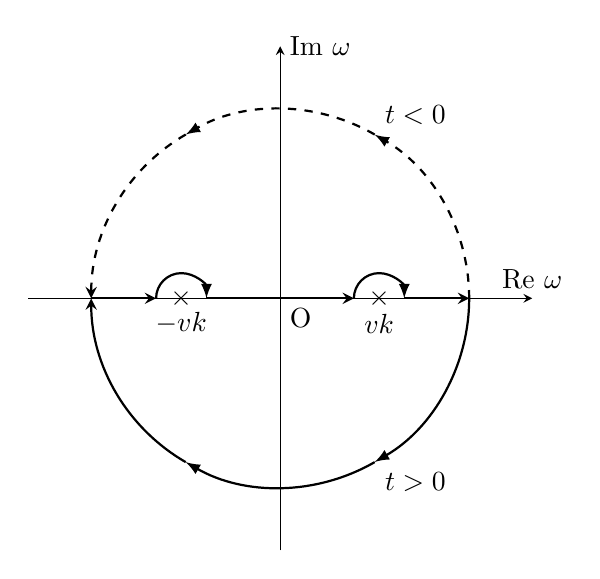
\begin{tikzpicture}[scale=0.8]
           \draw[->,>=stealth] (-4,0)--(4,0)node[above]{$\text{Re}\ \omega$}; %x軸
           \draw[->,>=stealth] (0,-4)--(0,4)node[right]{$\text{Im}\ \omega$}; %y軸
           \draw (0,0)node[below right]{O}; %原点
           \draw (-pi/2,-0)node[]{$\times$}; %点(-1,0)
           \draw (-pi/2,-0.4)node[]{$-vk$};
           \draw (pi/2,0)node[]{$\times$}; %点(0,1)
           \draw (pi/2,-0.4)node[]{$vk$};
           \draw [->,>=stealth,thick](-3,0)--(-1.97,0) ;
           \draw [->,>=stealth,thick](-1.17,0)--(1.17,0) ;
           \draw [->,>=stealth,thick](1.97,0)--(3,0) ;
           \draw [->,>=latex,thick](-1.97,0) arc (180:0:0.4);
          
           \draw [->,>=latex,thick](1.17,0) arc (180:0:0.4);

           \draw [->,>=latex,thick](3,0) arc (0:-60:3)node[below right]{$t>0$};
           \draw [->,>=latex,thick](1.5,-2.6) arc (-60:-120:3);
           \draw [->,>=stealth,thick](-1.5,-2.6) arc (-120:-180:3);

           \draw [->,>=latex,dashed,thick](3,0) arc (0:60:3)node[above right]{$t<0$};
           \draw [->,>=latex,dashed,thick](1.5,2.6) arc (60:120:3);
           \draw [->,>=stealth,dashed,thick](-1.5,2.6) arc (120:180:3);
            %\draw[domain=-1.22:1.22] plot(\x,{tan(\x r)})node[right]{$y=\tan x$};
          \end{tikzpicture}
       \caption{遅延グリーン関数の積分経路}
   \end{minipage}
   \begin{minipage}[b]{0.45\linewidth}
       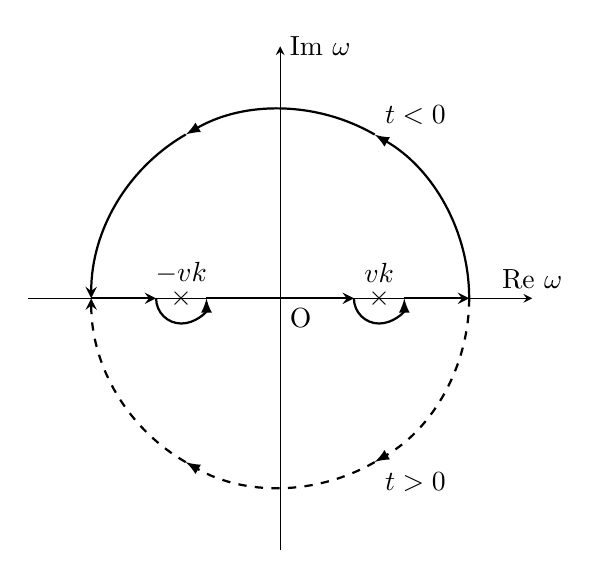
\begin{tikzpicture}[scale=0.8]
           \draw[->,>=stealth] (-4,0)--(4,0)node[above]{$\text{Re}\ \omega$}; %x軸
           \draw[->,>=stealth] (0,-4)--(0,4)node[right]{$\text{Im}\ \omega$}; %y軸
           \draw (0,0)node[below right]{O}; %原点
           \draw (-pi/2,-0)node[]{$\times$}; %点(-1,0)
           \draw (-pi/2,0.4)node[]{$-vk$};
           \draw (pi/2,0)node[]{$\times$}; %点(0,1)
           \draw (pi/2,0.4)node[]{$vk$};
           \draw [->,>=stealth,thick](-3,0)--(-1.97,0) ;
           \draw [->,>=stealth,thick](-1.17,0)--(1.17,0) ;
           \draw [->,>=stealth,thick](1.97,0)--(3,0) ;
           \draw [->,>=latex,thick](-1.97,0) arc (180:360:0.4);
          
           \draw [->,>=latex,thick](1.17,0) arc (180:360:0.4);

           \draw [->,>=latex,thick](3,0) arc (0:60:3)node[above right]{$t<0$};
           \draw [->,>=latex,thick](1.5,2.6) arc (60:120:3);
           \draw [->,>=stealth,thick](-1.5,2.6) arc (120:180:3);
           
           \draw [->,>=latex,dashed,thick](3,0) arc (0:-60:3)node[below right]{$t>0$};
           \draw [->,>=latex,dashed,thick](1.5,-2.6) arc (-60:-120:3);
           \draw [->,>=stealth,dashed,thick](-1.5,-2.6) arc (-120:-180:3);
           %\draw[domain=-1.22:1.22] plot(\x,{tan(\x r)})node[right]{$y=\tan x$};
          \end{tikzpicture}
          \caption{先進グリーン関数の積分経路}
   \end{minipage}
 \end{figure}


\begin{thebibliography}{99}
   \bibitem{ume} 梅村浩,『楕円関数論』,東京大学出版会,2000.
   \bibitem{tod} 戸田盛和,『楕円関数入門』,日本評論社,1991.
\end{thebibliography}

\end{document}
